% ****** Start of file apssamp.tex ******
%
%   This file is part of the APS files in the REVTeX 4.1 distribution.
%   Version 4.1r of REVTeX, August 2010
%
%   Copyright (c) 2009, 2010 The American Physical Society.
%
%   See the REVTeX 4 README file for restrictions and more information.
%
% TeX'ing this file requires that you have AMS-LaTeX 2.0 installed
% as well as the rest of the prerequisites for REVTeX 4.1
%
% See the REVTeX 4 README file
% It also requires running BibTeX. The commands are as follows:
%
%  1)  latex apssamp.tex
%  2)  bibtex apssamp
%  3)  latex apssamp.tex
%  4)  latex apssamp.tex
%
\documentclass[%
 reprint,
superscriptaddress,
%groupedaddress,
%unsortedaddress,
%runinaddress,
%frontmatterverbose, 
%preprint,
%showpacs,preprintnumbers,
%nofootinbib,
%nobibnotes,
%bibnotes,
 amsmath,amssymb,
 aps,
prc,
%prb,
%rmp,
%prstab,
%prstper,
%floatfix,
]{revtex4-1}

\usepackage{graphicx}% Include figure files
\usepackage{tabularx}
\newcolumntype{C}{>{\centering\arraybackslash}X}
\newcolumntype{L}{>{\raggedright\arraybackslash}X}%
\newcolumntype{R}{>{\raggedleft\arraybackslash}X}%
\usepackage{dcolumn}% Align table columns on decimal point
\usepackage{bm}% bold math
\usepackage{hyperref}% add hypertext capabilities
\usepackage[mathlines]{lineno}% Enable numbering of text and display math
%\linenumbers\relax % Commence numbering lines
\usepackage{circuitikz}
\usepackage{tikz}
\usepackage{xcolor}
\hypersetup{
    colorlinks,
    linkcolor={red!50!black},
    citecolor={blue!50!black},
    urlcolor={blue!80!black}
}
\usepackage{graphicx}
%\usepackage[showframe,%Uncomment any one of the following lines to test 
%%scale=0.7, marginratio={1:1, 2:3}, ignoreall,% default settings
%%text={7in,10in},centering,
%%margin=1.5in,
%%total={6.5in,8.75in}, top=1.2in, left=0.9in, includefoot,
%%height=10in,a5paper,hmargin={3cm,0.8in},
%]{geometry}
\usepackage{amsmath}
\usepackage{amssymb}
\begin{document}

\preprint{APS/123-QED}

\title{PGRE: Studying for Death?}% Force line breaks with \\

\author{Gray Ezequiel G.B. Perez}
\author{Schlack-Doggo}
\affiliation{%
 Reed College, 3203 SE Woodstock Blvd, Portland, OR 97202, USA
}%

\begin{abstract}
Attempting to avoid death by making a big study guide!
\end{abstract}
\maketitle
\tableofcontents
\section{Variable definitions}
% consistent variable definitions? or should this just be a list of standard ones?
\begin{enumerate}
\item[] $a\rightarrow$ acceleration

\item[] $c\rightarrow$ speed of light:\\
standard  $\approx 3*10^8\dfrac{m}{s}$

\end{enumerate}

\begin{figure}[t]
	\centering
	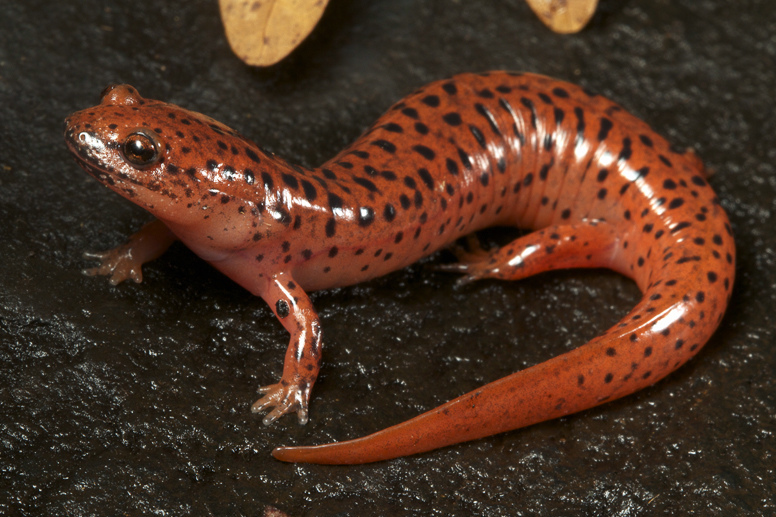
\includegraphics[width=0.48\textwidth]{figures/sally}
	\caption{Do figures work? Hell if I know. Here's a salamander.}
	\label{fig:sally}
\end{figure}

\section{Classical mechanics (20\%)}
% ETS description of the subject in brief
Such as kinematics, Newton's laws, work and energy, oscillatory motion, rotational motion about a fixed axis, dynamics of systems of particles, central forces and celestial mechanics, three-dimensional particle dynamics, Lagrangian and Hamiltonian formalism, noninertial reference frames, elementary topics in fluid dynamics.

\section{Electromagnetism (18\%)}
% ETS description of the subject in brief
Such as electrostatics, currents and DC circuits, magnetic fields in free space, Lorentz force, induction, Maxwell's equations and their applications, 
electromagnetic waves, AC circuits, magnetic and electric fields in matter.
\subsection{Electric Displacement Field}
On the shallow level the \textbf{Electric Displacement} is the equivalent of an electric field in a media. Specifically it is defined as:
$$\vec{D}\equiv \epsilon_0 \vec{E}+\vec{P}, $$
where $\vec{E}$ is the \textbf{electric field}, $\epsilon_0$ is the \textbf{vacuum permittivity}, and $\vec{P}$ is the \textbf{polarization}. Importantly 
the electric displacement appears in the in-media version of Maxwell's equations. Specifically,
$$\nabla \cdot D = \rho_f,$$
where $\rho_f$ is the \textbf{free charge density}, that which is not the \textbf{bound charge density}. We can prove this by first noting that $\rho_f$ and 
$\rho_b$ are two complementary subsets of the total charge density $\rho$ i.e.
$$\rho=\rho_f+ \rho_b.$$
next we not that the bound charge density is given by:
$$-\nabla\cdot\vec{P}=\rho_b.  $$
From this we get,
\begin{align*}
\nabla \cdot \vec{E} &=\dfrac{\rho}{\epsilon_0}\\
&=\dfrac{1}{\epsilon_0}\left(\rho_f-\nabla\cdot\vec{P}\right)\\
\nabla\cdot\left(\epsilon_0\vec{E}+\vec{P}\right)=\nablda\cdot\vec{D}&=\rho_f.
\end{align*}
if we limit ourselves to linear dielectrics according to the big G (or to wikipedia a linear, homogenous, isotropic dielectric with instantaneous response 
to changes in the electric field) we can define the polarization as:
$$\vec{P}=\epsilon_0\chi\vec{E}.$$
where $\chi$ is the \textbf{electric susceptibility} of the material. Now we define for our convenience and sorrow
$$\epsilon_r\equiv 1+\chi,$$
the \textbf{relative permittivity} of the material and
$$\epsilon=\epsilon_0\epsilon_r,$$
the \textbf{permittivity} of the material such that
$$\vec{D}=\epsilon\vec{E}.$$


\subsection{Maxwell's Equations}

\begin{itemize}
	\item \textbf{Speed of light:} The definition (in vacuum) can be found by taking the curl of Maxwell's equations and looking for something in the form of the wave equation. It is
	\begin{equation}
	    c=\frac{1}{\sqrt{\mu_0\epsilon_0}}.
	\end{equation}
	For light in matter, replace $\mu_0$ and $\epsilon_0$ with $\mu$ and $\epsilon$, respectively.
\end{itemize}

\subsection{Magnetic and Electric Fields in Matter}

\begin{itemize}
	\item \textbf{Permittivity:} In matter, the permittivity is given by
	\begin{equation}
		\epsilon = \kappa_E \epsilon_0,
	\end{equation}
	where $\epsilon$ is the absolute permittivity, $\kappa_E$ is the dielectric constant, and $\epsilon_0$ is vacuum permittivity. 
	
	If the applied field is not constant, then $\epsilon$ becomes frequency-dependent because the material's polarization does not change instantly. In this case
	\begin{equation}
		\epsilon (\omega) = \kappa_E\epsilon_0 - i \frac{\sigma}{\omega},
	\end{equation}
	where $\sigma$ is the conductivity of the material and $\omega$ is the frequency of the applied field.
	
	Note that electric susceptibility is related to the dielectric constant with the simple relation
	\begin{equation}
		\chi_E = \kappa_E - 1.
	\end{equation} 
	
	\item \textbf{Permeability:} The permeability is given by
	\begin{equation}
		\mu = \kappa_B \mu_0,
	\end{equation}
	where $\mu$ is the absolute permeability, $\kappa_B$ is a constant, and $\mu_0$ is vacuum permeability. $\kappa_B$ is related to the magnetic susceptibility by
	\begin{equation}
		\chi_B = \kappa_B - 1.
	\end{equation}
	
	Similarly to electric fields in matter, $\mu$ does have a frequency dependence. However, this dependence is negligible in non-magnetic materials.
	
	Fun fact: a material with $\mu < \mu_0$ is \textbf{diamagnetic}, and a material with $\mu > \mu_0$ is \textbf{paramagnetic}.
\end{itemize}


\section{Quantum Mechanics (12\%)}
% ETS description of the subject in brief
Such as fundamental concepts, solutions of the Schrödinger equation (including square wells, harmonic oscillators, and hydrogenic atoms), spin, angular 
momentum, wave function symmetry, elementary perturbation theory.

\section{Thermodynamics and Statistical Mechanics (10\%)}
% ETS description of the subject in brief
Such as the laws of thermodynamics, thermodynamic processes, equations of state, ideal gases, kinetic theory, ensembles, statistical concepts and calculation of thermodynamic quantities, thermal expansion and heat transfer.
\subsection{Thermodynamic Laws}
\subsubsection{1st Law}

\section{Atomic Physics (10\%)}
% ETS description of the subject in brief
Such as properties of electrons, Bohr model, energy quantization, atomic structure, atomic spectra, selection rules, black-body radiation, x-rays, atoms in electric and magnetic fields.

\section{Optics and Wave Phenomena (9\%)}
% ETS description of the subject in brief
Such as wave properties, superposition, interference, diffraction, geometrical optics, polarization, Doppler effect.

\subsection{Geometrical Optics}

\begin{figure}[t]
	\centering
	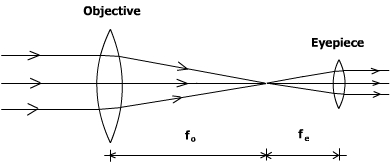
\includegraphics[width=0.48\textwidth]{figures/telescope}
	\caption{Ray diagram of a telescope. The objective has a focal length $f_\text{o}$ and the eyepiece has a focal length $f_\text{e}$. }
	\label{fig:telescope}
\end{figure}

\begin{itemize}
	\item \textbf{Optical Instruments:} In multi-lens instruments like telescopes or microscopes, the length $L$ of the instrument is equal to the sum of the focal lengths of the lenses. Figure \ref{fig:telescope} shows a ray diagram of a telescope. As is apparent in the figure,
	\begin{equation}
		f_\text{o} + f_\text{e} = L.
	\end{equation}
	If this were not the case, the image produced by the telescope would not be clear.
	
	The angular magnification $M$ of the instrument is given by the ratio
	\begin{equation}
		M = \left|\frac{f_\text{o}}{f_\text{e}}\right|.
	\end{equation}
\end{itemize}

\subsection{Doppler Effect}
The general form of the (classical) Doppler effect is
\begin{equation}
	f=\frac{c \pm v_\text{r}}{c \pm v_\text{s}} f_0,
\end{equation}
where $f$ is the observed frequency, $f_0$ is the source frequency, $c$ is the velocity of the waves in medium, $v_\text{r}$ is the velocity of the receiver relative to the medium, and $v_\text{s}$ is the velocity of the source relative to the medium. $v_\text{r}$ is positive if the receiver is moving towards the source and negative if it is moving away from the source. $v_\text{s}$ is positive if the source is moving away from the receiver and negative if it is towards the receiver.

In the relativistic case, the velocities above should be added using the velocity addition formula. This gives 
\begin{equation}
	f = \sqrt{\frac{1 - v/c}{1 + v/c}} f_0,
\end{equation}
where $v$ is the velocity of the source relative to the observer. $v$ is positive if the source and observer are receding from each other, and negative if the source and observer are approaching each other.

\section{Specialized Topics (9\%)}
% ETS description of the subject in brief
Nuclear and Particle physics (e.g., nuclear properties, radioactive decay, fission and fusion, reactions, fundamental properties of elementary particles), Condensed Matter (e.g., crystal structure, x-ray diffraction, thermal properties, electron theory of metals, semiconductors, superconductors), Miscellaneous (e.g., astrophysics, mathematical methods, computer applications)

\section{Special Relativity (6\%)}
% ETS description of the subject in brief
Such as introductory concepts, time dilation, length contraction, simultaneity, energy and momentum, four-vectors and Lorentz transformation, velocity addition.

\section{Laboratory Methods (6\%)}
% ETS description of the subject in brief
Such as data and error analysis, electronics, instrumentation, radiation detection, counting statistics, interaction of charged particles with matter, lasers and optical interferometers, dimensional analysis, fundamental applications of probability and statistics.

<<<<<<< HEAD
=======
\subsection{Error Analysis}
\begin{itemize}
	\item \textbf{Counting error:} the error in counting a sample of size $N$ is given by
	\begin{equation}
		\Delta N = \sqrt{N}.
	\end{equation}
\end{itemize}

\subsection{Instrumentation}
\begin{itemize}
	\item \textbf{Lasers:}
	\begin{itemize}
		\item \textit{Dye Laser:} Dye lasers use organic dye as a gain medium. Since the gain medium is a liquid, these lasers can be constructed in many different ways. They are very versatile, as they have high wavelength agility and the ability for high-energy pulses and high output power. This gives them many applications in science--they are used in spectroscopy and astronomy. According to Lucas, they can even be edible.
		
		\item \textit{Helium-Neon Laser:} The helium-neon (HeNe) laser uses a mixture of helium and neon gas as its gain medium. It is most commonly used for its 632.8 nm (red) output, although it can be tuned to other wavelengths. They are primarily used for research in optics labs due to their relatively low cost, ease of operation, and laser quality.
		
		\item \textit{Excimer Laser:} Excimer lasers (sometimes called exciplex lasers) are ultraviolet lasers. They are used in medical applications like eye surgery, as well as microelectronic devices and integrated circuits.
		
		\item \textit{Ruby Laser:} As the name suggests, this is a solid-state laser that uses a synthetic ruby crystal as its gain medium. They produce deep red pulses (694.3 nm) that are on the order of milliseconds. They are used to pump dye lasers and in research when short, red pulses are needed. They have other applications such as military rangefinding and hair removal, but in recent years they have been being replaced with more efficient Nd:YAG lasers.
		
		\item \textit{Nd:YAG Laser:} Neodymium-doped Yttrium Aluminum Garnet (Nd:YAG) lasers are solid-state lasers that use Nd:YAG as a gain medium. They typically emit infrared light at 1064 nm. They are one of the most commonly used lasers today, with applications in medicine, science, and industry. They are a popular choice for optical tweezers due to their infrared light. Since they are capable of producing fast, high-energy pulses, they are also used for laser-induced breakdown spectroscopy.
	\end{itemize}

	\item \textbf{Resolving Power:} The resolving power $R$ of a spectrometer is given by the ratio
	\begin{equation}
		R = \frac{\lambda}{\Delta\lambda},
	\end{equation}
	where $\lambda$ is the wavelength being observed and $\Delta\lambda$ is the minimum change in wavelength that the spectrometer can detect. For example, if a spectrometer observing at 500 nm cannot distinguish between 500 nm and 502 nm, then $\lambda = 500$ nm and $\Delta\lambda = 2$ nm, so $R = 250$.
\end{itemize}

>>>>>>> 06c0f1ca998ed5b831e8a2ac286255304c5d598a
\end{document}